\documentclass[12pt,letterpaper]{article}
\usepackage[legalpaper, margin=1in]{geometry}
\usepackage[numbers]{natbib}
\usepackage[urw-garamond]{mathdesign}
\usepackage[T1]{fontenc}

\title{Milestone 1 - SER502}
\author{\textbf{Team 10}\\ Kamal Penmetcha\\Karandeep Singh Grewal\\Nikhil Hiremath\\Subramanian Arunachalam}

\usepackage{tikz}
\usetikzlibrary{shapes.geometric, arrows}
\tikzstyle{block} = [rectangle, draw, fill=blue!10,
text width=5em, text centered, rounded corners, minimum height=4em]
\tikzstyle{line} = [draw, -latex']

\usepackage{hyperref}

\begin{document}

\maketitle

\section{About Developed Language}
\begin{tabular}{ll}
    Name      & IMPRO \\
    File Extension & .imp  \\
    Programming Paradigm & Imperative \\
    Github Repository & \href{https://github.com/kgrewal2/SER502-Spring2021-Team10}{github.com/kgrewal2/SER502-Spring2021-Team10}
\end{tabular}

\section{Project Pipeline}
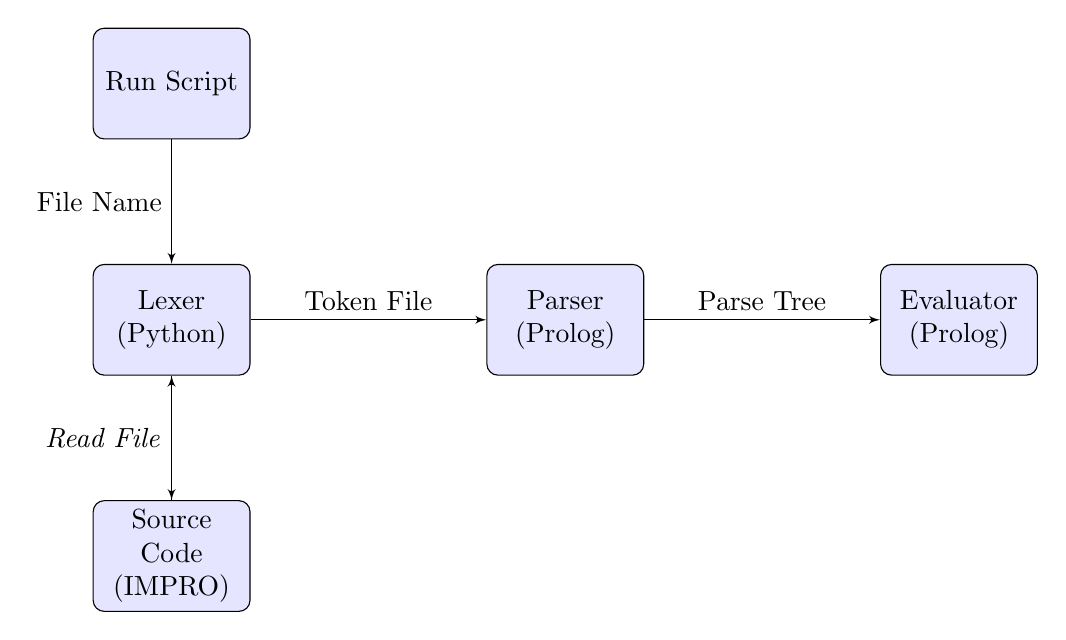
\begin{tikzpicture}
    \node [block] (bash) {Run Script};
    \node [block, below of=bash, node distance=3cm] (lexer) {Lexer\\(Python)};
    \node [block, below of=lexer, node distance=3cm] (source) {Source Code\\(IMPRO)};
    \node [block, right of=lexer, node distance=5cm] (parser) {Parser\\(Prolog)};
    \node [block, right of=parser, node distance=5cm] (evaluator) {Evaluator\\(Prolog)};
    \path [line] (bash) -- node [anchor=east] {File Name} (lexer);
    \path [line] (source) -- node [anchor=east] {\textit{Read File}} (lexer);
    \path [line] (lexer) -- node {} (source);
    \path [line] (lexer) -- node [anchor=south] {Token File} (parser);
    \path [line] (parser) -- node [anchor=south] {Parse Tree} (evaluator);
\end{tikzpicture}

\subsection{Run Script}
This will be a script that helps to run a IMPRO program file.
\subsection{Source Code}
This is the file that contains the code written in the developed language and needs to be executed.
\subsection{Lexer}
Lexer will accept the source code file (filename )as the input. It will break it into a list of tokens and will write to a new token file. The grammar of the developed language doesn't contain new line character. So we decided to use new line character as the separator for the tokens in the generated token file. The token file will contain each token put into a separate line (tokens are separated by a new line character).
\subsection{Parser}
This will read the file generated by the lexer and store the content of each line as separate element in a list. Then it will use the defined grammar rules to parse the list into a parse tree.
\subsection{Evaluator}
Evaluator will directly accept the parse tree generated by the parser and will start the evaluation process. It directly executes the instruction represented by the parse tree.

\section{Programming Languages Used}
\begin{tabular}{ll}
    \textbf{Component} & \textbf{Programming Language} \\
    Lexer & Python - \href{https://sly.readthedocs.io/en/latest/sly.html}{SLY (Sly Lex Yacc)} (Subject to change) \\
    Parser & Prolog \\
    Evaluator & Prolog
\end{tabular}

\section{Data Structures}
Data structure that will be used in the python lexer will be \textbf{LIST} and save it as a token file. This file is read by prolog parser and converted into a \textbf{LIST}. The parser then generates a parsetree \textbf{LIST} as the output. This output is accepted by the evaluator component and directly run on the machine. All the variables of the program executions are also stored as a prolog \textbf{LIST}.

\section{Parsing Technique}
Recursive Descent Parsing is a top-down parsing technique that turns all the non-terminals into a group of mutually recursive procedures based on the right hand side of the grammar rules. The rules of the parse are written in DCG.

\section{Design}
We aim to keep the syntax of our developed programming language to be a combination of C and Python. Example: We have taken the concept of braces from C whereas concept of a simpler print statement from Python. Different levels of grammar details are discussed in the following subsections.

\subsection{Program}
This is the top level unit of the code that will be written in our developed programming language. Any file that will be executed in our developed language will have the \texttt{Program} as the main structure.
\texttt{Program} consists of command list.

\subsection{Commands and Command List}
Commands are the building blocks for the \texttt{Program}. Commands are of two different types: Commands without block \& Commands with block. The term \texttt{block} will be discussed later. A set of one or more commands is called a command list. Each command without a block should end with a semi-colon symbol.
\begin{verbatim}
    print("Hello World");
    int i = a;
\end{verbatim}

\subsection{Block}
A set of one or more commands enclosed inside the curly brackets is called a block.

\begin{verbatim}
    {
        // commands
    }
\end{verbatim}

\subsection{Commands with block}
\subsubsection{For Loop}
\begin{verbatim}
    for(int i=0; i<10; i++){
        // commands
    }
\end{verbatim}

\subsubsection{While Loop}
\begin{verbatim}
    while(i<10){
        // commands
    }
\end{verbatim}

\subsubsection{For Loop (Enhanced)}
\begin{verbatim}
    for i in range(1, 10){
        // commands
    }
\end{verbatim}

\subsubsection{If}
\begin{verbatim}
    if(i==10){
        print("Ten");
    }
\end{verbatim}

\subsubsection{If Elif Else}
\begin{verbatim}
    if(i==10){
        print("Ten");
    }
    elif(i==1){
        print("One")
    }
    else{
        print("Not ten or zero")
    }
\end{verbatim}

\subsubsection{If Else}
\begin{verbatim}
    if(i==10){
        print("Ten");
    }
    else{
        print("Not Ten");
    }
\end{verbatim}

\subsection{Commands without block}
\subsubsection{Print}
\begin{verbatim}
    print("Your age is " + 10 + " years old");
\end{verbatim}

\subsubsection{Variable Declaration}
\begin{verbatim}
    int x;
\end{verbatim}

\subsubsection{Variable Assignment}
Uses equal to symbol for assignment operation
\begin{verbatim}
    x = 10;
\end{verbatim}

\subsection{Variable Naming}
\begin{itemize}
    \item Variable name can only start with lower case letter.
        \begin{verbatim}
            variable
        \end{verbatim}
    \item Variable name can contain lower case or upper case letter.
        \begin{verbatim}
            calculationAPI
            calculationModule
        \end{verbatim}
    \item Variable name can contain underscores.
        \begin{verbatim}
            calculation_API
            calculation_result
        \end{verbatim}
\end{itemize}

\subsection{Data Types}
\subsubsection{Integer}
\begin{verbatim}
    int x;
    x = 23;
\end{verbatim}

\subsubsection{Floating Point Numbers}
\begin{verbatim}
    float x;
    x = 100.23;
\end{verbatim}

\subsubsection{String}
\begin{verbatim}
    string x;
    string y;
    x = `hello';
    y = "there";
\end{verbatim}

\subsubsection{Boolean}
\begin{verbatim}
   bool x;
   x = True;
   x = False;
\end{verbatim}

\subsection{Operations}
\subsubsection{Addition}
Uses plus symbol
\begin{verbatim}
    x = 1 + 2 + a;
\end{verbatim}

\subsubsection{Subtraction}
Uses minus symbol
\begin{verbatim}
    x = 1 - 2 - a;
\end{verbatim}


\subsubsection{Multiplication}
Uses star symbol
\begin{verbatim}
    x = 1 * 2 * a;
\end{verbatim}


\subsubsection{Division}
Uses slash symbol
\begin{verbatim}
    x = 1 / 2;
\end{verbatim}

\subsubsection{Braces}
Uses braces' symbols
\begin{verbatim}
    x = 1 + (2 - 3 * (3 / 6));
\end{verbatim}

\subsubsection{Ternary Operator}
Uses question mark symbol and colon symbol
\begin{verbatim}
    int x = (i == 10) ? i + 10 : i - 10;
\end{verbatim}

\subsection{Reserved Keywords}
\begin{verbatim}
False  - Boolean Value
True   - Boolean Value
and    - Logical Operator
bool   - Variable Type
elif   - Conditional Command
else   - Conditional Command
float  - Variable Type
for    - Loop Command
if     - Conditional Command
in     - Checks if value is present in a list
int    - Variable
not    - Logical Operator
or     - Logical Operator
string - Variable Type
while  - Loop Command
\end{verbatim}

\subsection{Other potential features}
\begin{itemize}
    \item Multiple variable declaration in a single line.
        \begin{verbatim}
           int a, b, c;
        \end{verbatim}
    \item Variable assignment in the same command as variable declaration.
        \begin{verbatim}
           int a=10, b=20;
           int a=b=c=10;
        \end{verbatim}

    \item String version for enhanced for loop.
        \begin{verbatim}
           for character in string("Hello World"){
                print(character);
           }
        \end{verbatim}

    \item List Data Structure
        \begin{verbatim}
           x = [1, 2, "hello", 2.32];
        \end{verbatim}
\end{itemize}

\section{Contribution}
Link to \texttt{contribution.txt}\\
\href{https://github.com/kgrewal2/SER502-Spring2021-Team10/blob/main/contribution.txt}{\textit{https://github.com/kgrewal2/SER502-Spring2021-Team10/blob/main/contribution.txt}}

Milestone 1
- Design Document - Done by the whole team through various online meetings.

Project Level Future Contribution\\
\begin{tabular}{ll}
    Nikhil Hiremath & Lexer\\
    Kamal Penmetcha & Parser\\
    Karandeep Singh & Evaluator\\
    Subramanian     & Testing Scripts
\end{tabular}

\section{Grammar}
Notation Used: Prolog DCG \\
The implementation for the non-terminals like \texttt{number/2} will be done using prolog built-in predicates.
\begin{verbatim}
%%%%%%%%%%%%%%%%%
% NON-TERMINALS %
%%%%%%%%%%%%%%%%%

% Start Symbol
program --> command_list.

block --> ['{'], command_list, ['}'].

command_list --> command, command_list.
command_list --> command_without_block, command_list.
command_list --> command.
command_list --> command_without_block.

% Single Line Commands
command_without_block --> print_command.
command_without_block --> assignment_command.
command_without_block --> variable_declaration_command.

% Multi Line Commands
command --> for_loop_command.
command --> while_loop_command.
command --> for_enhanced_command.
command --> if_command.
command --> if_elif_else_command.
command --> if_else_command.

if_command --> if_part.
if_elif_else_command --> if_part, elif_part, else_part.
if_else_command --> if_part, else_part.

if_part --> ['if'], ['('], condition, [')'], block.
else_part --> ['else'], ['('], condition, [')'], block.
elif_part --> ['elif'], ['('], condition, [')'], block.
elif_part --> ['elif'], ['('], condition, [')'], block, elif_command.

while_loop_command --> ['while'], ['('], condition, [')'], block.

for_enhanced_command --> ['for'], variable_name, ['in'], ['range'],
    ['('], range_value, [','], range_value, [')'], block.


range_value --> variable_name | integer.

for_loop_command --> ['for'], ['('], assignment, [';'], condition, [';'],
    variable_change_part, [')'], block.

variable_change_part --> increment_expression.
variable_change_part --> decrement_expression.
variable_change_part --> variable_name, assignment_operator, expression.

condition --> expression, comparison_operators, expression.

decrement_expression --> variable_name, decrement_operator.
decrement_expression --> decrement_operator, variable_name.
increment_expression --> variable_name, increment_operator.
increment_expression --> increment_operator, variable_name.

print_command --> ['print'], ['('], expression, [')'], end_of_command.

expression --> value, operator, expression.
expression --> ['('], expression, [')'], operator, expression.
expression --> value.
expression --> ternary_expression.

ternary_expression --> ['('], condition, [')'], ['?'], expression, [':'],
    expression.

value --> float | integer | boolean_value | string_value | variable_name.

boolean_operators --> and_operator | or_operator | not_operator.

operators --> ['+'] | ['-'] | ['*'] | ['/'] | boolean_operators.

assignment_command --> variable_name, assignment_operator, expression,
    end_of_command.

variable_declaration_command --> variable_type, variable_name, end_of_command.
variable_declaration_command --> variable_type, variable_name, assignment_operator,
    expression, end_of_command.

variable_name --> lower_case, variable_name.
variable_name --> variable_name, upper_case.
variable_name --> variable_name, upper_case, variable_name.
variable_name --> variable_name, ['_'], variable_name.
variable_name --> lower_case.

string_value --> single_quote, character_phrase, single_quote.
string_value --> double_quote, character_phrase, double_quote.

character_phrase --> character, character_phrase.
character_phrase --> character.

character --> lower_case | upper_case | digit | symbol.

float --> integer, ['.'], integer.
float --> integer.

integer --> digit, integer.
integer --> digit.

%%%%%%%%%%%%%
% TERMINALS %
%%%%%%%%%%%%%
variable_type --> ['int'] | ['float'] | ['bool'] | ['string'].

decrement_operator --> ['--'].
increment_operator --> ['++'].

comparison_operators --> ['<'], ['>'], ['<='], ['>='], ['=='], ['!='].

single_quote --> ['\''].
double_quote --> ['\"'].

lower_case --> ['a'] | ['b'] | ['c'] | ['d'] | ['e'] | ['f'] | ['g'] |
    ['h'] | ['i'] | ['j'] | ['k'] | ['l'] | ['m'] | ['n'] | ['o'] | ['p'] |
    ['q'] | ['r'] | ['s'] | ['t'] | ['u'] | ['v'] | ['w'] | ['x'] | ['y'] |
    ['z'].

upper_case --> ['A'] | ['B'] | ['C'] | ['D'] | ['E'] | ['F'] | ['G'] |
    ['H'] | ['I'] | ['J'] | ['K'] | ['L'] | ['M'] | ['N'] | ['O'] | ['P'] |
    ['Q'] | ['R'] | ['S'] | ['T'] | ['U'] | ['V'] | ['W'] | ['X'] | ['Y'] |
    ['Z'].

symbol --> [' '] | ['!'] | ['\"'] | ['#'] | ['$'] | ['%'] | ['&'] |
    ['\''] | ['('] | [')'] | ['*'] | ['+'] | [','] | ['-'] | ['.'] | ['/'] |
    [':'] | [';'] | ['<'] | ['='] | ['>'] | ['?'] | ['@'] | ['['] | ['\\'] |
    [']'] | ['^'] | ['_'] | ['`'] | ['{'] | ['|'] | ['}'] | ['~'].

digit --> ['0'] | ['1'] | ['2'] | ['3'] | ['4'] | ['5'] | ['6'] | ['7'] |

       ['8'] | ['9'].

boolean_value --> ['True'].
boolean_value --> ['False'].

assignment_operator --> [‘=’].
end_of_command --> [‘;’].

and_operator --> ['and'].
or_operator --> ['or'].
not_operator --> ['not'].

\end{verbatim}

\end{document}
